\chapter{راهنمای استفاده از الگوی لاتک دانشگاه صنعتی امیرکبیر(پلی‌تکنیک تهران)}

\section{مقدمه}
حروف‌چینی پروژه کارشناسی، پایان‌نامه یا رساله یکی از موارد پرکاربرد استفاده از زی‌پرشین است. از طرفی، یک پروژه، پایان‌نامه یا رساله،  احتیاج به تنظیمات زیادی از نظر صفحه‌آرایی  دارد که ممکن است برای
یک کاربر مبتدی، مشکل باشد. به همین خاطر، برای راحتی کار کاربر، یک کلاس با نام 
\verb;AUTthesis;
 برای حروف‌چینی پروژه‌ها، پایان‌نامه‌ها و رساله‌های دانشگاه صنعتی امیرکبیر با استفاده از نرم‌افزار زی‌پرشین،  آماده شده است. این فایل به 
گونه‌ای طراحی شده است که کلیه خواسته‌های مورد نیاز  مدیریت تحصیلات تکمیلی دانشگاه صنعتی امیرکبیر را برآورده می‌کند و نیز، حروف‌چینی بسیاری
از قسمت‌های آن، به طور خودکار انجام می‌شود.

کلیه فایل‌های لازم برای حروف‌چینی با کلاس گفته شده، داخل پوشه‌ای به نام
\verb;AUTthesis;
  قرار داده شده است. توجه داشته باشید که برای استفاده از این کلاس باید فونت‌های
  \verb;Nazanin B;،
 \verb;PGaramond;
 و
  \verb;IranNastaliq;
    روی سیستم شما نصب شده باشد.
\section{این همه فایل؟!}\label{sec2}
از آنجایی که یک پایان‌نامه یا رساله، یک نوشته بلند محسوب می‌شود، لذا اگر همه تنظیمات و مطالب پایان‌نامه را داخل یک فایل قرار بدهیم، باعث شلوغی
و سردرگمی می‌شود. به همین خاطر، قسمت‌های مختلف پایان‌نامه یا رساله  داخل فایل‌های جداگانه قرار گرفته است. مثلاً تنظیمات پایه‌ای کلاس، داخل فایل
\verb;AUTthesis.cls;، 
تنظیمات قابل تغییر توسط کاربر، داخل 
\verb;commands.tex;،
قسمت مشخصات فارسی پایان‌نامه، داخل 
\verb;fa_title.tex;,
مطالب فصل اول، داخل 
\verb;chapter1;
و ... قرار داده شده است. نکته مهمی که در اینجا وجود دارد این است که از بین این  فایل‌ها، فقط فایل 
\verb;AUTthesis.tex;
قابل اجرا است. یعنی بعد از تغییر فایل‌های دیگر، برای دیدن نتیجه تغییرات، باید این فایل را اجرا کرد. بقیه فایل‌ها به این فایل، کمک می‌کنند تا بتوانیم خروجی کار را ببینیم. اگر به فایل 
\verb;AUTthesis.tex;
دقت کنید، متوجه می‌شوید که قسمت‌های مختلف پایان‌نامه، توسط دستورهایی مانند 
\verb;input;
و
\verb;include;
به فایل اصلی، یعنی 
\verb;AUTthesis.tex;
معرفی شده‌اند. بنابراین، فایلی که همیشه با آن سروکار داریم، فایل 
\verb;AUTthesis.tex;
است.
در این فایل، فرض شده است که پایان‌نامه یا رساله شما، از5 فصل و یک پیوست، تشکیل شده است. با این حال، اگر
  پایان‌نامه یا رساله شما، بیشتر از 5 فصل و یک پیوست است، باید خودتان فصل‌های بیشتر را به این فایل، اضافه کنید. این کار، بسیار ساده است. فرض کنید بخواهید یک فصل دیگر هم به پایان‌نامه، اضافه کنید. برای این کار، کافی است یک فایل با نام 
\verb;chapter6;
و با پسوند 
\verb;.tex;
بسازید و آن را داخل پوشه 
\verb;AUTthesis;
قرار دهید و سپس این فایل را با دستور 
\texttt{\textbackslash include\{chapter6\}}
داخل فایل
\verb;AUTthesis.tex;
و بعد از دستور
\texttt{\textbackslash include\{chapter6\}}
 قرار دهید.

\section{از کجا شروع کنم؟}
قبل از هر چیز، بدیهی است که باید یک توزیع تِک مناسب مانند 
\verb;Live TeX;
و یک ویرایش‌گر تِک مانند
\verb;Texmaker;
را روی سیستم خود نصب کنید.  نسخه بهینه شده 
\verb;Texmaker;
را می‌توانید  از سایت 
 \href{http://www.parsilatex.com}{پارسی‌لاتک}%
\LTRfootnote{\url{http://www.parsilatex.com}}
 و
\verb;Live TeX;
را هم می‌توانید از 
 \href{http://www.tug.org/texlive}{سایت رسمی آن}%
\LTRfootnote{\url{http://www.tug.org/texlive}}
 دانلود کنید.
 
در مرحله بعد، سعی کنید که  یک پشتیبان از پوشه 
\verb;AUTthesis;
 بگیرید و آن را در یک جایی از هارددیسک سیستم خود ذخیره کنید تا در صورت خراب کردن فایل‌هایی که در حال حاضر، با آن‌ها کار می‌کنید، همه چیز را از 
 دست ندهید.
 
 حال اگر نوشتن پایان‌نامه اولین تجربه شما از کار با لاتک است، توصیه می‌شود که یک‌بار به طور سرسری، کتاب «%
\href{http://www.tug.ctan.org/tex-archive/info/lshort/persian/lshort.pdf}{مقدمه‌ای نه چندان کوتاه بر
\lr{\LaTeXe}}\LTRfootnote{\url{http://www.tug.ctan.org/tex-archive/info/lshort/persian/lshort.pdf}}»
   ترجمه دکتر مهدی امیدعلی، عضو هیات علمی دانشگاه شاهد را مطالعه کنید. این کتاب، کتاب بسیار کاملی است که خیلی از نیازهای شما در ارتباط با حروف‌چینی را برطرف می‌کند.
 
 
بعد از موارد گفته شده، فایل 
\verb;AUTthesis.tex;
و
\verb;fa_title;
را باز کنید و مشخصات پایان‌نامه خود مثل نام، نام خانوادگی، عنوان پایان‌نامه و ... را جایگزین مشخصات موجود در فایل
\verb;fa_title;
 کنید. دقت داشته باشید که نیازی نیست 
نگران چینش این مشخصات در فایل پی‌دی‌اف خروجی باشید. فایل 
\verb;AUTthesis.cls;
همه این کارها را به طور خودکار برای شما انجام می‌دهد. در ضمن، موقع تغییر دادن دستورهای داخل فایل
\verb;fa_title;
 کاملاً دقت کنید. این دستورها، خیلی حساس هستند و ممکن است با یک تغییر کوچک، موقع اجرا، خطا بگیرید. برای دیدن خروجی کار، فایل 
\verb;fa_title;
 را 
\verb;Save;، 
(نه 
\verb;As Save;)
کنید و بعد به فایل 
\verb;AUTthesis.tex;
برگشته و آن را اجرا کنید. حال اگر می‌خواهید مشخصات انگلیسی پایان‌نامه را هم عوض کنید، فایل 
\verb;en_title;
را باز کنید و مشخصات داخل آن را تغییر دهید.%
\RTLfootnote{
برای نوشتن پروژه کارشناسی، نیازی به وارد کردن مشخصات انگلیسی پروژه نیست. بنابراین، این مشخصات، به طور خودکار،
نادیده گرفته می‌شود.
}
 در اینجا هم برای دیدن خروجی، باید این فایل را 
\verb;Save;
کرده و بعد به فایل 
\verb;AUTthesis.tex;
برگشته و آن را اجرا کرد.

برای راحتی بیشتر، 
فایل 
\verb;AUTthesis.cls;
طوری طراحی شده است که کافی است فقط  یک‌بار مشخصات پایان‌نامه  را وارد کنید. هر جای دیگر که لازم به درج این مشخصات باشد، این مشخصات به طور خودکار درج می‌شود. با این حال، اگر مایل بودید، می‌توانید تنظیمات موجود را تغییر دهید. توجه داشته باشید که اگر کاربر مبتدی هستید و یا با ساختار فایل‌های  
\verb;cls;
 آشنایی ندارید، به هیچ وجه به این فایل، یعنی فایل 
\verb;AUTthesis.cls;
دست نزنید.

نکته دیگری که باید به آن توجه کنید این است که در فایل 
\verb;AUTthesis.cls;،
سه گزینه به نام‌های
\verb;bsc;,
\verb;msc;
و
\verb;phd;
برای تایپ پروژه، پایان‌نامه و رساله،
طراحی شده است. بنابراین اگر قصد تایپ پروژه کارشناسی، پایان‌نامه یا رساله را دارید، 
 در فایل 
\verb;AUTthesis.tex;
باید به ترتیب از گزینه‌های
\verb;bsc;،
\verb;msc;
و
\verb;phd;
استفاده کنید. با انتخاب هر کدام از این گزینه‌ها، تنظیمات مربوط به آنها به طور خودکار، اعمل می‌شود.

\section{مطالب پایان‌نامه را چطور بنویسم؟}
\subsection{نوشتن فصل‌ها}
همان‌طور که در بخش 
\ref{sec2}
گفته شد، برای جلوگیری از شلوغی و سردرگمی کاربر در هنگام حروف‌چینی، قسمت‌های مختلف پایان‌نامه از جمله فصل‌ها، در فایل‌های جداگانه‌ای قرار داده شده‌اند. 
بنابراین، اگر می‌خواهید مثلاً مطالب فصل ۱ را تایپ کنید، باید فایل‌های 
\verb;AUTthesis.tex;
و
\verb;chapter1;
را باز کنید و محتویات داخل فایل 
\verb;chapter1;
را پاک کرده و مطالب خود را تایپ کنید. توجه کنید که همان‌طور که قبلاً هم گفته شد، تنها فایل قابل اجرا، فایل 
\verb;AUTthesis.tex;
است. لذا برای دیدن حاصل (خروجی) فایل خود، باید فایل  
\verb;chapter1;
را 
\verb;Save;
کرده و سپس فایل 
\verb;AUTthesis.tex;
را اجرا کنید. یک نکته بدیهی که در اینجا وجود دارد، این است که لازم نیست که فصل‌های پایان‌نامه را به ترتیب تایپ کنید. می‌توانید ابتدا مطالب فصل ۳ را تایپ کنید و سپس مطالب فصل ۱ را تایپ کنید.

نکته بسیار مهمی که در اینجا باید گفته شود این است که سیستم
\lr{\TeX},
محتویات یک فایل تِک را به ترتیب پردازش می‌کند. به عنوان مثال، اگه فایلی، دارای ۴ خط دستور باشد، ابتدا خط ۱، بعد خط ۲، بعد خط ۳ و در آخر، خط ۴ پردازش می‌شود. بنابراین، اگر مثلاً مشغول تایپ مطالب فصل ۳ هستید، بهتر است
که دو دستور
\verb~\chapter{مقدمه}
خریداری یا استفاده از یک محصول با این پیش‌زمینه و تفکر که محصول مورد نظر نیاز خاصی را برطرف خواهد کرد، خود به خود انتظار برطرف کردن نیازمندی‌های ذهن مصرف‌کننده را در وی می‌انگیزد
\cite{___1389}.
در ابتدا شاید صرفا رفع نیاز مصرف‌کنندگان، به هر روش ممکن - و نه الزاما با بالاترین کیفیت - دغدغه اصلی تولیدکننده باشد اما به مرور و با گذشت زمان که نیازمندی‌ها پخته‌تر می‌شوند و ارتقا می‌یابند، کیفیت نیز در آن‌ها دخیل می‌شود. از طرفی، وجود نام‌ونشان‌های متعدد و متنوع در بسیاری از صنایع نیز، منجر به ایجاد رقابت میان فعالان هر عرصه شده است؛ رقابتی که کیفیت تعیین‌کننده‌ترین عامل برد و باخت در آن است
\cite{pressman_software_2015}.
صنعت نرم‌افزار نیز، به عنوان یکی از صنایع نوین که محصولاتش امروزه سهم قابل توجهی از بازار را در مصارف روزمره اداری و شخصی به خود اختصاص داده است، از این قاعده مستثنی نیست. بنابراین در تولید و توسعه یک محصول نرم‌افزاری نیز به منظور موفقیت هرچه بیشتر، می‌بایست به کیفیت، نگاه جدی داشته باشیم.\\
به طور خاص، در سامانه‌های کاربردی مبتنی بر وب\RTLfootnote{Web Applications} و موبایل که جامعه کاربریشان هر روز بیشتر و بیشتر می‌شود، نیازمندی‌های مختلفی در طول چرخه عمر نرم‌افزار بروز پیدا می‌کنند. از طرفی در دنیای نرم‌افزار،  گسترده‌تر شدن دامنه دسترسی به یک محصول نرم‌افزاری، الزاماتی برای آن فراهم می‌آورد که برای مثال، می‌توان گفت محصول نرم‌افزاری می‌بایست توسط یک فرد عادی از جامعه هدف مشتریان، قابل استفاده باشد. قابل استفاده بودن و استفاده‌پذیری را نه در دانش فنی کاربران سیستم، بلکه در قابل فهم بودن رابط میان سیستم و کاربران تعریف می‌کنیم
\cite{albert_measuring_2013}.\\
البته ناگفته نماند دانش فنی و مهارت استفاده از ابزارهای فناوری‌محور، بخش غیرقابل اغماضی از توانایی استفاده از یک محصول نرم‌افزاری را ممکن می‌سازد؛ ولی امروزه، در مورد محصولات و سامانه‌های نرم‌افزاری تحت وب که به طور معمول با تعداد کاربران زیادی مواجه هستند، قابل استفاده بودن و استفاده‌پذیری آن‌ها در هنگام کار یک کاربر عادی، یکی از معیارهای مهم کیفیتی به شمار می‌رود.
\section{کیفیت در نرم‌افزار}
کیفیت یک نرم‌افزار، یک خصیصه ثابت و مشخص کلی نیست. بلکه به انتظارات و نیازمندی‌های ذی‌نفعان بستگی زیادی دارد؛ برای قرار دادن کیفیت در اولویت‌های تولید نرم‌افزار، می‌بایست، در همان ابتدای کار و قبل از شروع هرچیز دیگری، یک تعریف مدون و کاملا مشخص از کیفیت داشته باشیم.\\
\begin{figure}[H]
	\centering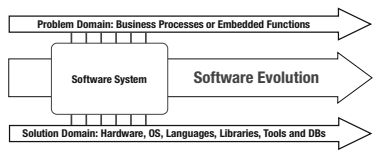
\includegraphics[width=9cm]{Resources/mediator.PNG}
	\caption[نرم‌افزار به عنوان پلی بین دامنه مسئله و دامنه راه‌حل]
	{نرم‌افزار به عنوان پلی بین دامنه مسئله و دامنه راه‌حل
		\cite{wagner_software_2013}؛
		توسعه در یک دامنه، به طور خودکار توسعه در دامنه دیگر را می‌طلبد و در نتیجه می‌باید از فناوری‌ها و تکنولوژی‌ها به نحو احسنت بهره جست تا نیازهای حوزه مسئله را منطبق بر سیستم‌ها و ماشین‌های به روز کرد.
	}
	\label{fig:mediator}
\end{figure}
بسیاری از تحقیقات در سال‌های گذشته، صرف به دست آوردن فرآیندهای نرم‌افزاری با کیفیت شده است؛ البته که فرآیندهای باکیفیت در نهایت منجر به تولید محصولی با کیفیت می‌شود، ولی برای بروز کیفیت در فرآیندها نیز خصیصه‌های کیفی محصول نرم‌افزاری هدف، باید به طور مشخص قید شوند
\cite{sommerville_software_2016}.
هرچند که داشتن یک تعریف مدون و مشخص از کیفیت، لازمه کار هر فرآیند مهندسی نرم‌افزار است، نکته حائز اهمیتی که بسیاری از محققین و پژوهشگران در آثار خود از جمله آقایان پرسمن
\cite{pressman_software_2015}،
سامرویل
\cite{sommerville_software_2016}
و واگنر
\cite{wagner_software_2013}
به آن اشاره کرده‌اند، بیانگر این موضوع است که داشتن یک توصیف کیفیتی  کامل و دقیق از سیستم هدف نیز، به تنهایی، کافی نیست؛ چرا که همین توصیف کیفیتی نیز با گذر زمان، دچار تغییر و تحول خواهد شد و دیگر نیازمندی‌های کیفیتی، معتبر نخواهند بود.\\
همانطور که در شکل
\ref{fig:mediator}
ملاحظه می‌شود، نرم‌افزار میان دو دامنه مسئله و راه‌حل ارتباط برقرار می‌کند و می‌بایست پلی بین فرآیند‌های کسب‌وکاری و پلتفرم‌های فناوری (سیستم‌های عامل، سخت‌افزارها و نرم‌افزارهای مختلف) ایجاد کند. اما توجه به این نکته حائز اهمیت است که هم فرآیندهای کسب‌وکار و هم پلتفرم‌های فناوری، در طول زمان دچار تغییر می‌شوند؛ به خصوص که سرعت تغییرات در عصر حاضر به شدت زیاد است. سخت‌افزارها منسوخ می‌شوند، سیستم‌های عامل به نسخه‌های جدیدتری ارتقا پیدا می‌کنند، زبان‌های برنامه‌نویسی پیشرفته‌تر می‌شوند، ابزارهای جدیدی تولید می‌شوند و کسب‌وکارها در نتیجه این تغییرات، خود را به روز می‌کنند و فرآیندهای کسب‌وکاری نیز می‌بایست بتوانند این تغییرات را پشتیبانی کنند و در نتیجه تغییر می‌کنند
\cite{wagner_software_2013}.\\
در نتیجه ویژگی‌ها و نیازمندی‌های کیفی نرم‌افزار نیز تغییر پیدا می‌کند و اگر خود نرم‌افزار مطابق این تغییرات به روز رسانی نشود، سیستم کم‌کیفیتی خواهیم داشت.
\subsection{تضمین و کنترل کیفیت}
همانطور که پرسمن در کتابش
\cite{pressman_software_2015}
مطرح می‌کند، رسیدن به یک محصول با کیفیت در مهندسی نرم‌افزار، به صورت ضمنی و خود به خود ممکن نیست؛ بلکه نتیجه بازنگری در چهار بعد کلی در فرآیند مهندسی نرم‌افزار و اِعمال مجموعه آن‌ها است:
\begin{itemize}
	\item 
	روش‌های مهندسی نرم‌افزار
	\item 
	تکنیک‌های مدیریت پروژه
	\item 
	فعالیت‌های کنترل کیفیت
	\item
	فعالیت‌های تضمین کیفیت
\end{itemize}
طبق این اظهار نظر، با فرض اِعمال شدن روش‌های درست و بهره‌ور مهندسی نرم‌افزار و تکنیک‌های موثر در مدیریت پروژه تولید نرم‌افزار - که با تقریب خوبی هر دو را می‌توان جزو روش‌های مدیریتی و در حوزه تصمیم‌گیری‌های کلان سیستم دانست - بدیهی است که همچنان کنترل کیفیت و تضمین آن، دو بعد فنی و جزئی‌تر رسیدن به نرم‌افزار با کیفیت را تشکیل می‌دهند. بنابراین می‌بایست روش‌های موثر به منظور انجام فرایند‌های کنترل کیفیت و تضمین رسیدن به آن، توسط تیم مهندسی نرم‌افزار اتخاذ شود.\\
اما، مشابه هر فرایند و فعالیت دیگری، رسیدن به کیفیت نیز هزینه‌های خاص خود را دارد. هزینه کیفیت در نرم‌افزار، مطابق اظهارنظر پرسمن، به سه دسته هزینه‌های پیش‌گیری، هزینه‌های ارزیابی و هزینه‌های خرابی تقسیم می‌شود. هرکدام از این هزینه‌ها، در صورت پیش‌بینی و رفع نواقص محتمل/پیش‌آمده در هر مرحله از طراحی و پیاده‌سازی، بدون اینکه وارد مرحله بعدی شویم، می‌تواند با نرخ بسیار زیادی کاهش یابد 
\cite{pressman_software_2015}.
%\subsection{نقش ابزارها در تامین کیفیت}
%صثثقلثقل
\subsection{کیفیت در سامانه‌های نرم‌افزاری مبتنی بر وب}
یکی از علل عدم رضایت کاربران و مشتریان از وب‌اپلیکیشن‌ها - که درنتیجه این نارضایتی، آمار کاربران وب‌اپلیکیشن‌های کسب‌وکارها دستخوش تغییرات نامطلوب شده و حتی هزینه‌های گزافی به تیم مهندسی نرم‌افزار به خاطر اعمال تغییر پس از تحویل، وارد می‌شود- طراحی نه‌چندان کاربرپسندانه واسط کاربری و زیبایی آن‌هاست 
\cite{agarwal_assessing_2002}؛
بدیهی است که استفاده از مدل‌های فرایندی چابک  و تکراری می‌تواند در کاهش هزینه‌های طراحی مجدد پس از تحویل و یا اعمال تغییر در رابط‌های موجود، موثر باشد
\cite{pressman_software_2015}،
 اما هنوز یک سوال بدون پاسخ خواهد ماند:
 \textit{«چه رابطی برای کاربران وب‌اپلیکیشن (محصول) من مناسب است و طبق نیازمندی‌های فعلی حداکثر کیفیت را تامین خواهد کرد؟»}
 برای پاسخ به این سوال، چک‌لیست‌ها و توصیه‌های فراوانی ارائه شده است
  \cite{pressman_software_2015, sommerville_software_2016}
 که هرکدام به نحوی در افزایش کیفیت رابط‌های کاربری تاثیرگذار بوده‌اند، اما برای تست یک رابط کاربری به صورت کمی، تحلیل و یافتن نقاط ضعف در زیبایی و همچنین ریزبینی در مورد استفاده‌پذیری یک واسط کاربری، به نظر می‌رسد که بررسی بیشتری مورد نیاز است
 \cite{albert_measuring_2013}.
 
 \section{مشخصه‌های کیفی نرم‌افزار}
 \subsection{کارآیی}
 به تعبیر نویسندگان مرجع
 \cite{albert_measuring_2013}
هر کاربر می‌تواند برای خودش تعریفی از کارآیی ارائه نماید. در ادامه بررسی مفصل و مقایسه تطبیقی از مدل‌های کیفی مختلف و کارآیی در هرکدام انجام شده است ولی در اینجا به طور مختصر به ارائه و مقایسه سه نوع دیدگاه از تعریف کارآیی می‌پردازیم:
\begin{enumerate}
	\item 
	سازمان بین‌المللی استانداردها (ایزو ۹۲۴۱-۱۱) کارآیی را در سه حوزه تعریف می‌کند:
	\emph{«میزان سودی که استفاده از یک محصول در رسیدن به اهداف مورد نظر کاربران در رابطه با کاربردی مشخص، که همراه با تاثیرگذاری، بهره‌وری و رضایت باشد، کارآیی آن محصول نامیده می‌شود.»}
	\item
	جامعه متخصصین کارآیی
	\LTRfootnote{Usability Professionals Association}
	بیشتر روی فرایند تولید و توسعه محصول تمرکز می‌کنند و با بیان استفاده‌پذیری به عنوان «یک روش برای کاستن هزینه‌ها و تولید ابزارهایی که مختص کاربرانشان باشد»، از ویژگی مرتبط بودن همواره استفاده‌پذیری با کاربران، استفاده می‌کند.
	\item 
	استیو کورگ در کتاب خود، کاری نکن که من به فکر کردن بیفتم  تعریف عامیانه‌تری را ارائه می‌دهد؛ وی معتقد است که استفاده‌پذیری به معنی اطمینان حاصل کردن از کار کردن خوب محصول نهایی است. با این توضیح که یک فرد با دانش، توانمندی و تجربه کم نیز بایستی بتواند از محصول به راحتی استفاده کند و نیازهای خود را برطرف سازد.
\end{enumerate}
 با بررسی‌های مرجع
 \cite{albert_measuring_2013}
 تمامی تعاریف مطرح برای استفاده‌پذیری، شامل سه زمینه کلیدی و مهم هستند:
 \begin{enumerate}
 	\item 
 	کاربری وجود دارد.
 	\item 
 	این کاربر مشغول انجام کاری است.
 	\item 
 	کاربر در حین کار خود، با یک سیستم یا محصول نرم‌افزاری در تعامل است.
 \end{enumerate}
 یکی از عوامل بسیار تاثیرگذار در استفاده‌پذیری هر محصولی، رابط کاربری آن است؛ از طرفی وجهی که در طرف کاربران قرار دارد و کاربران با آن‌ در ارتباط هستند، در کاربردهای حساس، اهمیتی دو چندان می‌یابد.به عنوان مثال تابلویی که در شکل
\ref{fig:bluffton}
قابل مشاهده است به دلیل استفاده‌پذیر نبودن منجر به تلفات جانی شده. طبق اظهاراتی که در مرجع 
\cite{albert_measuring_2013}
از این حادثه شده است، گرچه استفاده‌پذیری در ابتدا موردی سطحی و غیر ضروری به نظر می‌رسد اما عدم وجود آن در برخی از کاربردهای حساس می‌تواند منجر به آسیب‌ها و خسارت‌های زیادی شود.
\begin{figure}[H]
	\centering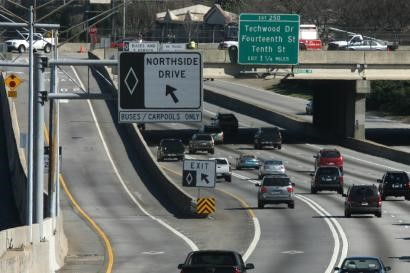
\includegraphics[width=14.8cm]{Resources/tabloo.JPG}
	\caption[تابلویی که نصب نامناسب آن منجر به عدم استفاده‌پذیری و تصادف جاده‌ای شد]
	{تابلویی که نصب نامناسب آن منجر به عدم استفاده‌پذیری و تصادف جاده‌ای شد؛ این تابلو (تابلوی بزرگ سفیدرنگ) که به خاطر نصب در جای نامناسب و استفاده‌پذیری پایینش، راه منتهی به مسیری را نشان می‌دهد که یک طرفه است و در اصل هدف از قرار دادن این تابلو، نشان دادن خروجی در چند متر جلوتر بود
		\cite{noauthor_bluffton_2018}.
	}
	\label{fig:bluffton}
\end{figure}
 اینکه کاربر در طول دوره کاری‌اش با سیستم به طور دقیق به چه موارد منفی یا مثبت یا حتی خنثی برخورده، نقش مهمی در تجربه کاربری وی خواهد داشت.\\
 استفاده‌پذیری به طور کلی به توانایی کاربر در انجام موفق یک کار مشخص دلالت دارد، در حالی که تجربه کاربری به جنبه وسیع‌تری پرداخته و شامل احساسات، عواطف و ادراکات کاربر در حین کار با سیستم می‌شود
 \cite{albert_measuring_2013}.
 در بخش‌های بعدی و با بررسی مدل‌های کیفی مختلف که به منظور سنجش کمی کیفیت نرم‌افزار ارائه شده‌اند، خواهیم دید که استفاده‌پذیری نرم‌افزار، به عنوان یکی از مشخصه‌های اصلی در اغلب این مدل‌ها و به صورت صریح  بیان شده است. با بررسی پژوهش‌ها و کارهای گذشته و همچنین نکاتی از مرجع
 \cite{pressman_software_2015}،
 می‌توان گفت از سال ۱۹۷۰ تا به اکنون، تقریبا در هر مدل کیفی ارائه شده برای نرم‌افزار و به طور خاص برای سامانه‌های کاربری تحت وب، استفاده‌پذیری به صورت صریح به عنوان یک مشخصه اصلی بیان شده است؛ بنابراین می‌توان ادعا کرد استفاده‌پذیری یک نرم‌افزار، از جمله ویژگی‌های مهم کیفی در دستیابی و کنترل کیفیت نرم‌افزار است.
 \subsubsection{استفاده‌پذیری و لایه‌های طراحی سامانه‌های مبتنی بر وب}
 استفاده‌پذیری در وب‌اپلیکیشن‌ها - که امروزه نقش مهمی در ارائه محتوا و سرویس به کاربران دارند - به عنوان یکی از ابعاد و مشخصه‌های اصلی و مهم در کیفیت مطرح است
 \cite{pressman_software_2015}.
رسیدن به کیفیت بالا نیازمند صرف هزینه (تلاش و زمان) است؛ صرفا با در نظر گرفتن بعد کارآیی، پرواضح است که هرچه مشکلات و نواقص رابط‌های کاربری زودتر پیدا شده و مرتفع گردند، با پرداخت هزینه (تلاش و زمان) کمتر به کیفیت بیشتری رسیده‌ایم؛ لایه‌های طراحی سامانه‌های مبتنی بر وب، هر کدام تمرکز جدایی دارند که در ادامه به طور مختصر قید شده‌اند. هر کدام از این لایه‌ها، به نوعی کارآیی نهایی محصول را تامین می‌کنند و در تضمین کیفیت باید به هر لایه به طور جداگانه توجه ویژه‌ای را معطوف نمود.
\section{چرخه طراحی سامانه‌های مبتنی بر وب}
از جمله مراحل هرم طراحی وب‌اپلیکیشن
\cite{pressman_software_2015}،
طراحی واسط کاربری است.  همانطور که در شکل
\ref{fig:pyramid}
مشاهده می‌شود، طراحی زیبایی، محتوا، پیمایش، معماری و همچنین مولفه نیز در فرایند طراحی می‌بایست انجام شوند که هرکدام نکات خاص خود را دارند و می‌توانند در استفاده‌پذیری سامانه کاربردی مبتنی بر وب تاثیرگذار باشند.
\begin{figure}[H]
	\centering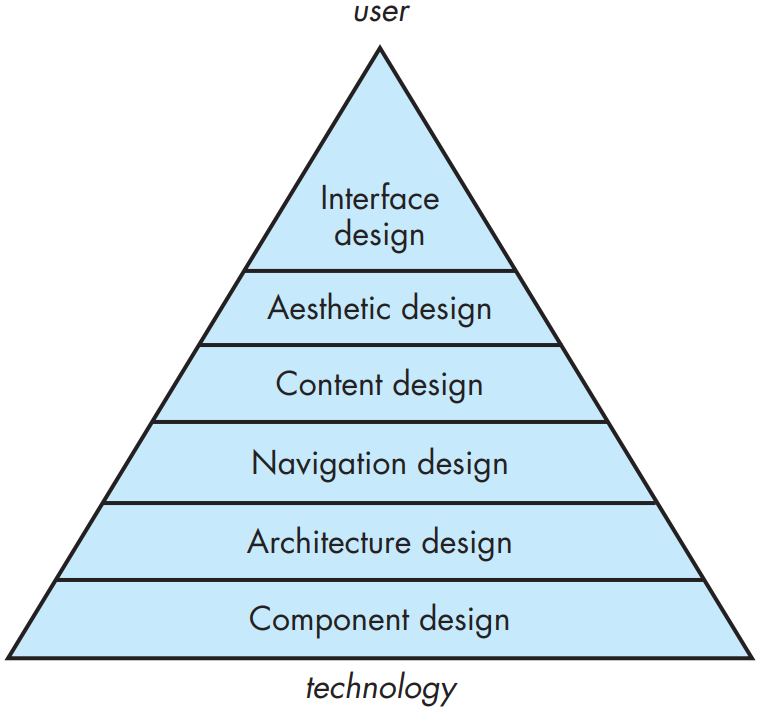
\includegraphics[width=7cm]{Resources/pyramid.PNG}
	\caption[هرم طراحی سامانه‌های مبتنی بر وب]
	{هرم طراحی سامانه‌های مبتنی بر وب
		\cite{pressman_software_2015}
		که نشان‌دهنده لایه‌ها، مراحل و اجزای ساخت یک سامانه مبتنی بر وب است.
	}
	\label{fig:pyramid}
\end{figure}
همچنین شایان ذکر است که لایه‌های مختلف این هرم، هرکدام توجه جداگانه‌ای دارند و می‌بایست در تامین کیفیت، به در هر لایه سیاست‌های به خصوصی اتخاذ شود. قبل از تولید کد وب‌اپلیکیشن، واسط کاربری، به صورت یک نمونه اولیه و در قالب طرح‌های ابتدایی، ماکت‌های مفهومی و یا چارچوب‌های کلی توصیف و طراحی می‌شوند. پس از رسیدن به توافق با مشتری (در صورت نیاز) و یا اعمال تغییرات متعدد تا رسیدن به توافق، این طراحی به کد قابل اجرا و پیاده‌سازی روی وب‌اپلیکیشن تبدیل می‌شود و نهایتا به تولید واسط کاربری آن می‌انجامد
\cite{sommerville_software_2016}.

\begin{figure}[H]
	\centering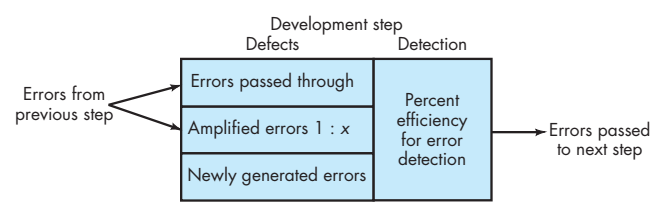
\includegraphics[width=12cm]{Resources/defect.PNG}
	\caption[مدل تشدید خرابی در نرم‌افزار]
	{مدل تشدید خرابی در نرم‌افزار
		\cite{pressman_software_2015}
		نشان‌دهنده تاثیرگذاری خرابی‌های مراحل قبل در هر مرحله از توسعه محصول می‌باشد. طبق این مدل، هرچه بتوان درصد بیشتری از خطاها را هنگام مرور و بررسی هر مرحله شناخت، خرابی‌های کمتری به مراحل بعدی راه پیدا کرده و در نتیجه محصول نهایی با کیفیت‌تر خواهد بود.
	}
	\label{fig:defect}
\end{figure}
مطابق شکل
\ref{fig:defect}
خرابی‌ها و خطاها در صورتی که برطرف نشوند و وارد مرحله بعد شوند، می‌توانند در تولید وب‌اپلیکیشن مشکلات جدی‌ای ایجاد کنند؛ چرا که این خطاها تشدید می‌شوند و دچار خرابی کار سایر لایه‌ها نیز می‌گردند و در نهایت منجر به افت کیفیت محصولات نهایی می‌گردند. از جمله خطاها و خرابی‌های مطرح در حوزه طراحی رابط کاربری، ناکارآمد بودن ایده‌های اولیه و چکش‌نخورده است. مطابق آنچه در قسمت تضمین و کنترل کیفیت گفته شد، در صورت ارزیابی، تحلیل و رفع ایرادات مربوط به استفاده‌پذیری رابط کاربری، در همان مراحل ابتدایی و پس از تولید نمونه‌ اولیه، می‌توان هزینه‌های بعدی را به طور قابل ملاحظه‌ای کمتر کرد.\\
مانند هر روش کیفی دیگری در تضمین کیفیت نرم‌افزار، به منظور دستیابی به استفاده‌پذیری قابل قبول (مطابق نیازهای مشتری) در واسط کاربری وب‌اپلیکیشن‌ها (همچون هر مشخصه اصلی دیگری) می‌بایست فاکتورها، معیارها و مولفه‌های مختلفی به منظور خرد و قابل اندازه‌گیری کردن این مفهوم کلان مطرح شود؛ به طوری که بتوان در قالب مقادیر کمی، نیازمندی‌ها را با داده‌های به دست آمده از ارزیابی رابط کاربری وب‌اپلیکیشن مقایسه و تحلیل کرد. اما در بسیاری از موارد، همانطور که
\cite{agarwal_assessing_2002,p._miguel_review_2014, albert_measuring_2013}
ذکر می‌کنند، حقیقت محض و یا تخمینی تضمین‌کننده‌ای\RTLfootnote{Promising Heuristic}، برای رسیدن به یک رابط کاربری «خوب» وجود ندارد و طراحی‌های استفاده‌پذیر و موثر، موفقیت خود را اغلب یا به روش‌های تجربی، که الزاماً با روش‌های علمی به اثبات نرسیده‌اند، و یا به ذوق هنری طراح مدیون‌اند.
\subsection{تلفیق نگاه مهندسی و هنری}
دور از ذهن نیست که بگوییم یکی از فاکتورهای محبوبیت یک اثر هنری، جذابیت اثر در دید مخاطبانش است. بنابراین پرواضح است که در مورد رابط‌های کاربری، که در ابتدای کار و هنگامی که هنوز توسعه سامانه در فازهای ابتدایی و مذاکرات ابتدایی است به صورت یک طرح مفهومی بوده و اثر یک طراح -که الزاما شاید سررشته‌ای از مهندسی نداشته باشد- هستند، نظر کاربران و استفاده کنندگان آن طرح مفهومی و نحوه تعاملشان با طرح مفهومی، یکی از مشخصه‌های تعیین‌کننده برای موفقیت رابط کاربریِ هدف و تضمین کیفیت آن است.\\
در نتیجه به نظر می‌رسد اندازه‌گیری نظرات کاربران و داشتن یک دید مهندسی در نقطه نظرات کاربران و واکنش‌های آن‌ها هنگام کار با یک طرح مفهومی که به منظور استفاده در یک رابط کاربری ساخته شده است، امری لازم و مثبت خواهد بود و درکل منجر به افزایش اطلاعات تیم طراح و تیم توسعه از نیازهای کاربران خواهد شد.
\section{جمع‌سپاری}
تا سال ۲۰۱۲، با بررسی‌های مرجع 
\cite{estelles-arolas_towards_2012}،
حدود ۴۰ تعریف مختلف در مقالات و پژوهش‌های علمی، حتی گاهی تعاریف متناقض با هم، برای جمع‌سپاری ارائه شده است. نویسندگان آن اثر، با درنظر گرفتن ابعاد مطرح در تعاریف مختلف، در نهایت تعریف نسبتا مفصلی از این مفهوم ارائه می‌دهند که ترجمه آزاد آن در ادامه ذکر شده است: 
\paragraph{جمع‌سپاری}
که ترجمه شده عبارت
\lr{Crowdsourcing}
است، نوعی فعالیت برخط
\LTRfootnote{Online}
مشارکتی است که طی آن یک فرد، یا یک سازمان با ابزارهای کافی به گروهی از افراد با سطح دانش متغیر و گونه‌های متفاوت و با تعداد نامعلومی به انجام فعالیت‌هایی می‌پردازند. در این کار دو سر برد، کارگران انجام دهنده کار
\LTRfootnote{Crowd Workers}
به دلیل داوطلبانه بودن مشارکتشان، از انجام کار خود احساس رضایت می‌کنند؛ چه به خاطر پولی که در ازای انجام کار دریافت می‌کنند و چه به خاطر توسعه مهارت‌های شخصی و یا سایر انگیزه‌ها؛ افراد جمع‌سپارنده هم از مشارکت افراد در حل مسائل پیچیده کمک جسته و سودآوری خود را خواهند داشت. \\
یکی از انگیزه‌های استفاده از جمع‌سپاری، جمع‌آوری داده
\LTRfootnote{Data Collection}
است. در این استفاده، از کارگران جمع‌سپاری شده بهره گرفته می‌شود تا بتوان به مجموعه عظیمی از دیتاست‌ها و یا داده‌های جدید دست پیدا کرد.
\subsection{جمع‌سپاری برای جمع‌آوری داده}
انگیزه اصلی استفاده از جمع‌سپاری در این پروژه، جمع‌آوری داده است. ابزار هدف، قادر خواهد بود تا با استفاده از جمع‌سپاری، بتواند نتایج تست‌های تعریف‌شده توسط مشتریان را از کارگران جمع‌آوری کرده و روی آن‌ها تحلیل و پردازش انجام دهد. عدم وجود یک حقیقت محض قابل اتکا
\LTRfootnote{Ground Truth}
در رابطه با خوب بودن و یا بد بودن یک طراحی رابط کاربری و سلیقه‌ای بودن آن، مهم‌ترین انگیزه استفاده از جمع‌سپاری است؛ همچنین مبتنی بودن تصمیمات و داده‌ها بر داده‌های کاربران مخاطب، می‌تواند منجر به موفقیت حداکثری یک محصول در سازمان شود.\\
همچنین به عنوان یک مهندس، همواره بر آنیم که روش‌های مهندسی و رویکردهای قابل تکرار داشته باشیم. بنابراین نتیجه تلاش در استفاده از یک روش مهندسی برای مدیریت نظرات، استفاده از جمع سپاری خواهد بود.
~
و
\verb~\chapter{طریقه‌ی مرجع نویسی و واژه‌نامه‌}
\section{طریقه‌ی مرجع نویسی}
برای نوشتن مراجع پایان نامه، برای راحتی کار به صورت زیر عمل می‌کنیم:
\subsection{بارگیری مراجع}
در ابتدا مراجع را باید از سایت‌های معتبر بارگیری کنیم، مثلا برای ارجاع دادن به مقاله‌ی
\lr{A classification of some Finsler connections and their applications}
ابتدا به سایت
\href{scholar.google.com}{گوگل اسکولار} 
رفته و این مقاله را جستجو می‌کنیم. پس از پیدا کردن این مقاله، مانند شکل زیر، در زیر نام و چکیده‌ی مقاله، $5$ گزینه وجود دارد که عبارتند از:\\

\begin{enumerate}
\item \lr{ Cited by}

\item \lr{ Related articles}

\item \lr{ All 6 versions}

\item \lr{ Cite}

\item \lr{ Save}
\end{enumerate}
\begin{figure}[!h]
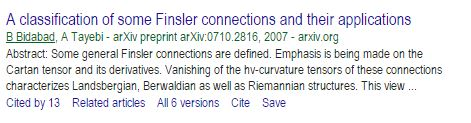
\includegraphics[height=3cm]{bidabad}
\caption{نمونه یک مقاله در گوگل اسکولار}
\end{figure}
در اینجا ما به گزینه‌ی چهارم یعنی
\lr{ Cite}
احتیاج داریم. بر روی آن کلیک کرده و پنجره‌ای مانند
\cref{fig.2}
باز می‌شود که دارای $4$ گزینه‌ی زیر است:
\begin{enumerate}
\item \lr{BibTeX}

\item \lr{EndNote}

\item \lr{RefMan}

\item \lr{RefWorks}
\end{enumerate}
\begin{figure}
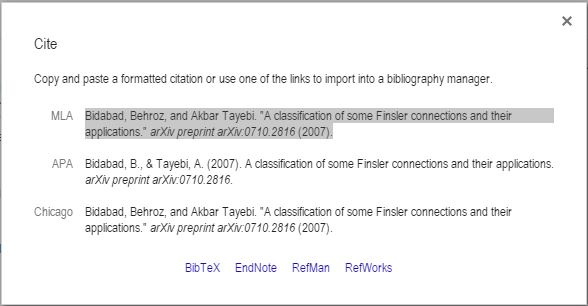
\includegraphics[scale=.6]{bibref}
\caption{پنجره‌ی باز شده در گوگل اسکولار}\label{fig.2}
\end{figure}
روی گزینه‌ی اول، یعنی
\verb;BibTeX;
کلیک کرده و همه‌ی نوشته‌های پنجره‌ی باز شده را مانند زیر، کپی کرده و در فایل
\verb;references.bib;
موجود در فایل
\verb;AUTthesis;
پیست می‌کنیم. سپس کلیدهای
\verb;Ctrl+s;
را می‌زنیم تا فایل ذخیره شود.\\
\begin{latin}
	\normalsize
\begin{verbatim}
@ article{bidabad2007classification,
title={A classification of some Finsler connections and their applications},
author={Bidabad, Behroz and Tayebi, Akbar},
journal={arXiv preprint arXiv:0710.2816},
year={2007}
}
\end{verbatim}
\end{latin}
\subsection{روش ارجاع در متن}
برای ارجاع دادن به مقاله‌ی بالا، باید در جایی که می‌خواهید ارجاع دهید، دستور زیر را تایپ کنید:
\begin{latin}
\lr{$\backslash$cite\{bidabad2007classification\}}
\end{latin}
همانطور که مشاهده می‌کنید از کلمه‌ای که در سطر اول ادرس مقاله آمده (یعنی کلمه‌ی پس از
\lr{@article$\lbrace$})
استفاده کرده‌ایم. پس از دستور فوق، به صورت \cite{bidabad2007classification} و \cite{aa} مرجع خواهد خورد. توجه شود که در صورتی مراجع چاپ خواهند شد که در متن به انها ارجاع داده شده باشد. همچنین برای ارجاع چندتایی از دستور 
\lr{$\backslash$cite\{name1, name2,...\}}
استفاده کنید که به‌صورت \cite{najafi2008finsler, zakeri, najafi} ارجاع خواهند خورد.
\subsection{روش اجرای برنامه}
ابتدا فایل
\verb;AUT_thesis.tex;
را باز کرده و آن را دو بار اجرا کنید. سپس حالت اجرا را از 
\verb;Build Quick;
به حالت
\verb;Bibtex;
تغییر داده و دوباره برنامه را اجرا کنید. دو بار دیگر برنامه را در حالت 
\verb;Build Quick;
اجرا کرده و نتیجه را مشاهده کنید. در این روش تمامی مراجع بر اساس اینکه کدام یک در متن زودتر به آن ارجع داده شده لیست خواهند شد.
\subsection{مراجع فارسی}
برای نوشتن مراجع فارسی باید به صورت دستی، در همان فایل قبلی به صورت زیر عمل می‌کنیم:
\begin{LTR}
\noindent\verb;@article{manifold,;\\
\verb;title={;منیفلد هندسه\verb;},;\\
\verb;author={;بیدآباد دکتربهروز \verb;},;\\
\verb;journal{; امیرکبیر صنعتی دانشگاه\verb;},;\\
\verb;year={1389},;\\
\verb;LANGUAGE={Persian};\\
\verb;};
\end{LTR}
همانطور که مشاهده می‌کنید تنها تفاوت آن با حالت مراجع انگلیسی، سطر آخر آن می‌باشد که زبان را مشخص می‌کند که حتماً باید نوشته شود.
\section{راهنمای واژه‌نامه}

به دلیل پیچیدگی واژه‌نامه‌های موجود در سایت پارسی لاتک، از روش زیر برای نوشتن واژه‌نامه استفاده کنید:

ابتدا با استفاده از اکسل، واژه های خود را یک‌بار براساس حروف الفبای فرسی و بار دیگر انگلیسی مرتب کنید. سپس واژه ها را در فایل \lr{dicen2fa} و \lr{dicfa2en} قرار دهید.

\section{ساخت نمایه}\label{Namaye}
\subsection{ساخت نمایه}
 \begin{enumerate}

\item
کلمات مورد نظر خود مثلا \lr{word} با دستور \verb|\index{word}| ایندکس کنید.
\item
نحوه‌ی اجرای \lr{Make Index}   در ویرایشگرهای \lr{TeX Maker} و \lr{TeX Works}:
\begin{itemize}
\item  تک‌میکر: از منوی \lr{Tools} گزینه‌ی \lr{Xindy Make Index} را کلیک کنید یا از دکمه‌‌های میانبر \lr{Ctrl+Alt+I} استفاده کنید.

\item  تک‌ورکز: ابتدا باید مثل عکس زیر تنظیم  و سپس گزینه‌ی \lr{Xindy Make Index}  انتخاب و روی دکمه‌ی سبز رنگ کلیک کنید یا از دکمه‌های  \lr{Ctrl+T} استفاده کنید.

\begin{figure}[!h]
\centerline{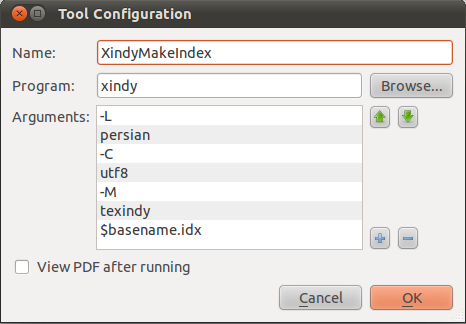
\includegraphics[width=.5\textwidth]{Xindy_Make_Index.png}}
\caption{تنظیمات مربوط به تک‌ورکز}
\end{figure}

\end{itemize}
 \end{enumerate}
 
 \index{کتاب}
\index{پارسی‌لاتک}
\index{بی‌دی}
\index{سوال}
\index{عنصر}
\index{گزینه}
\index{ژاکت}
\index{مرکز دانلود}
\index{اجرا}
\index{تک‌لایو}
\index{ثالث}
\index{جهان}
\index{چهار}
\index{حمایت}
\index{خواهش}
\index{دنیا}
\index{زی‌پرشین}
\index{ریحان}
\index{شیرین}
\index{صمیمی}
\index{ضمیر}
\index{طبیب}~
را در فایل 
\verb~AUTthesis.tex~،
غیرفعال%
\RTLfootnote{
برای غیرفعال کردن یک دستور، کافی است پشت آن، یک علامت
\%
 بگذارید.
}
 کنید. زیرا در غیر این صورت، ابتدا مطالب فصل ۱ و ۲ پردازش شده (که به درد ما نمی‌خورد؛ چون ما می‌خواهیم خروجی فصل ۳ را ببینیم) و سپس مطالب فصل ۳ پردازش می‌شود و این کار باعث طولانی شدن زمان اجرا می‌شود. زیرا هر چقدر حجم فایل اجرا شده، بیشتر باشد، زمان بیشتری هم برای اجرای آن، صرف می‌شود.

\subsection{مراجع}
برای وارد کردن مراجع به فصل 2
مراجعه کنید.
\subsection{واژه‌نامه فارسی به انگلیسی و برعکس}
برای وارد کردن واژه‌نامه فارسی به انگلیسی و برعکس، بهتر است مانند روش بکار رفته در فایل‌های 
\verb;dicfa2en;
و
\verb;dicen2fa;
عمل کنید.

\section{اگر سوالی داشتم، از کی بپرسم؟}
برای پرسیدن سوال‌های خود در مورد حروف‌چینی با زی‌پرشین،  می‌توانید به
 \href{http://forum.parsilatex.com}{تالار گفتگوی پارسی‌لاتک}%
\LTRfootnote{\url{http://www.forum.parsilatex.com}}
مراجعه کنید. شما هم می‌توانید روزی به سوال‌های دیگران در این تالار، جواب بدهید.
